\section{SEM}

	Das für diese Untersuchung verwendete Rasterelektronenmikroskop (Hitachi S-4000), detektiert mit einem SE-Detektor die Sekundärelektronen.
	Zusätzlich kann zeitgleich das Röntgen-Absorptionsspektrum der untersuchten Probe aufgenommen werden.

	Zunächst werden verschiedene Beispielproben unter dem Mikroskop betrachtet und dann eine der zuvor hergestellten Proben untersucht, damit die Auflösungsgrenze bestimmt werden kann.
	Daraufhin wird das Spektrum einer Messingprobe aufgenommen und mit denen einer Kupfer- und einer Zinkprobe verglichen, um den jeweiligen Gehalt in dem Messing zu bestimmen.
	Zuletzt wird eine Probe mit vier unbekannten Elementen betrachtet.
	Dafür sollen die auftretenden Elemente anhand ihrer Absorptionsspektren bestimmt werden und eine Karte der Elemente angefertigt werden.

\subsection{Beispielproben und Auflösungsgrenze} % TODO Text

	\begin{figure}[ht]
		\centering
		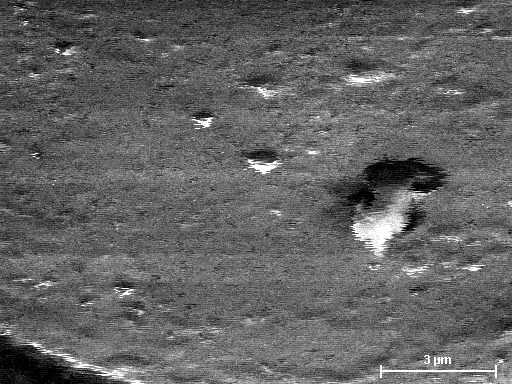
\includegraphics[width=.35\textwidth]{raw/SEM/Hummelauge_M9010}
		\caption{SEM-Bild eines Hummelauges bei einer Vergrößerung von x9010.}
		\label{fig:Hummelaugex9010}
	\end{figure}

	\

	...

\subsection{Untersuchung einer Messingprobe}

	Die zu untersuchende Messingprobe befindet sich wie auch die Kupfer- und die Zinkprobe an verschiedenen Stellen der gleichen Halterung.
	Beispielhaft ist dies in \cref{fig:messing_halterung} dargestellt.
	\begin{wrapfigure}{r}{.5\textwidth}
		\centering
		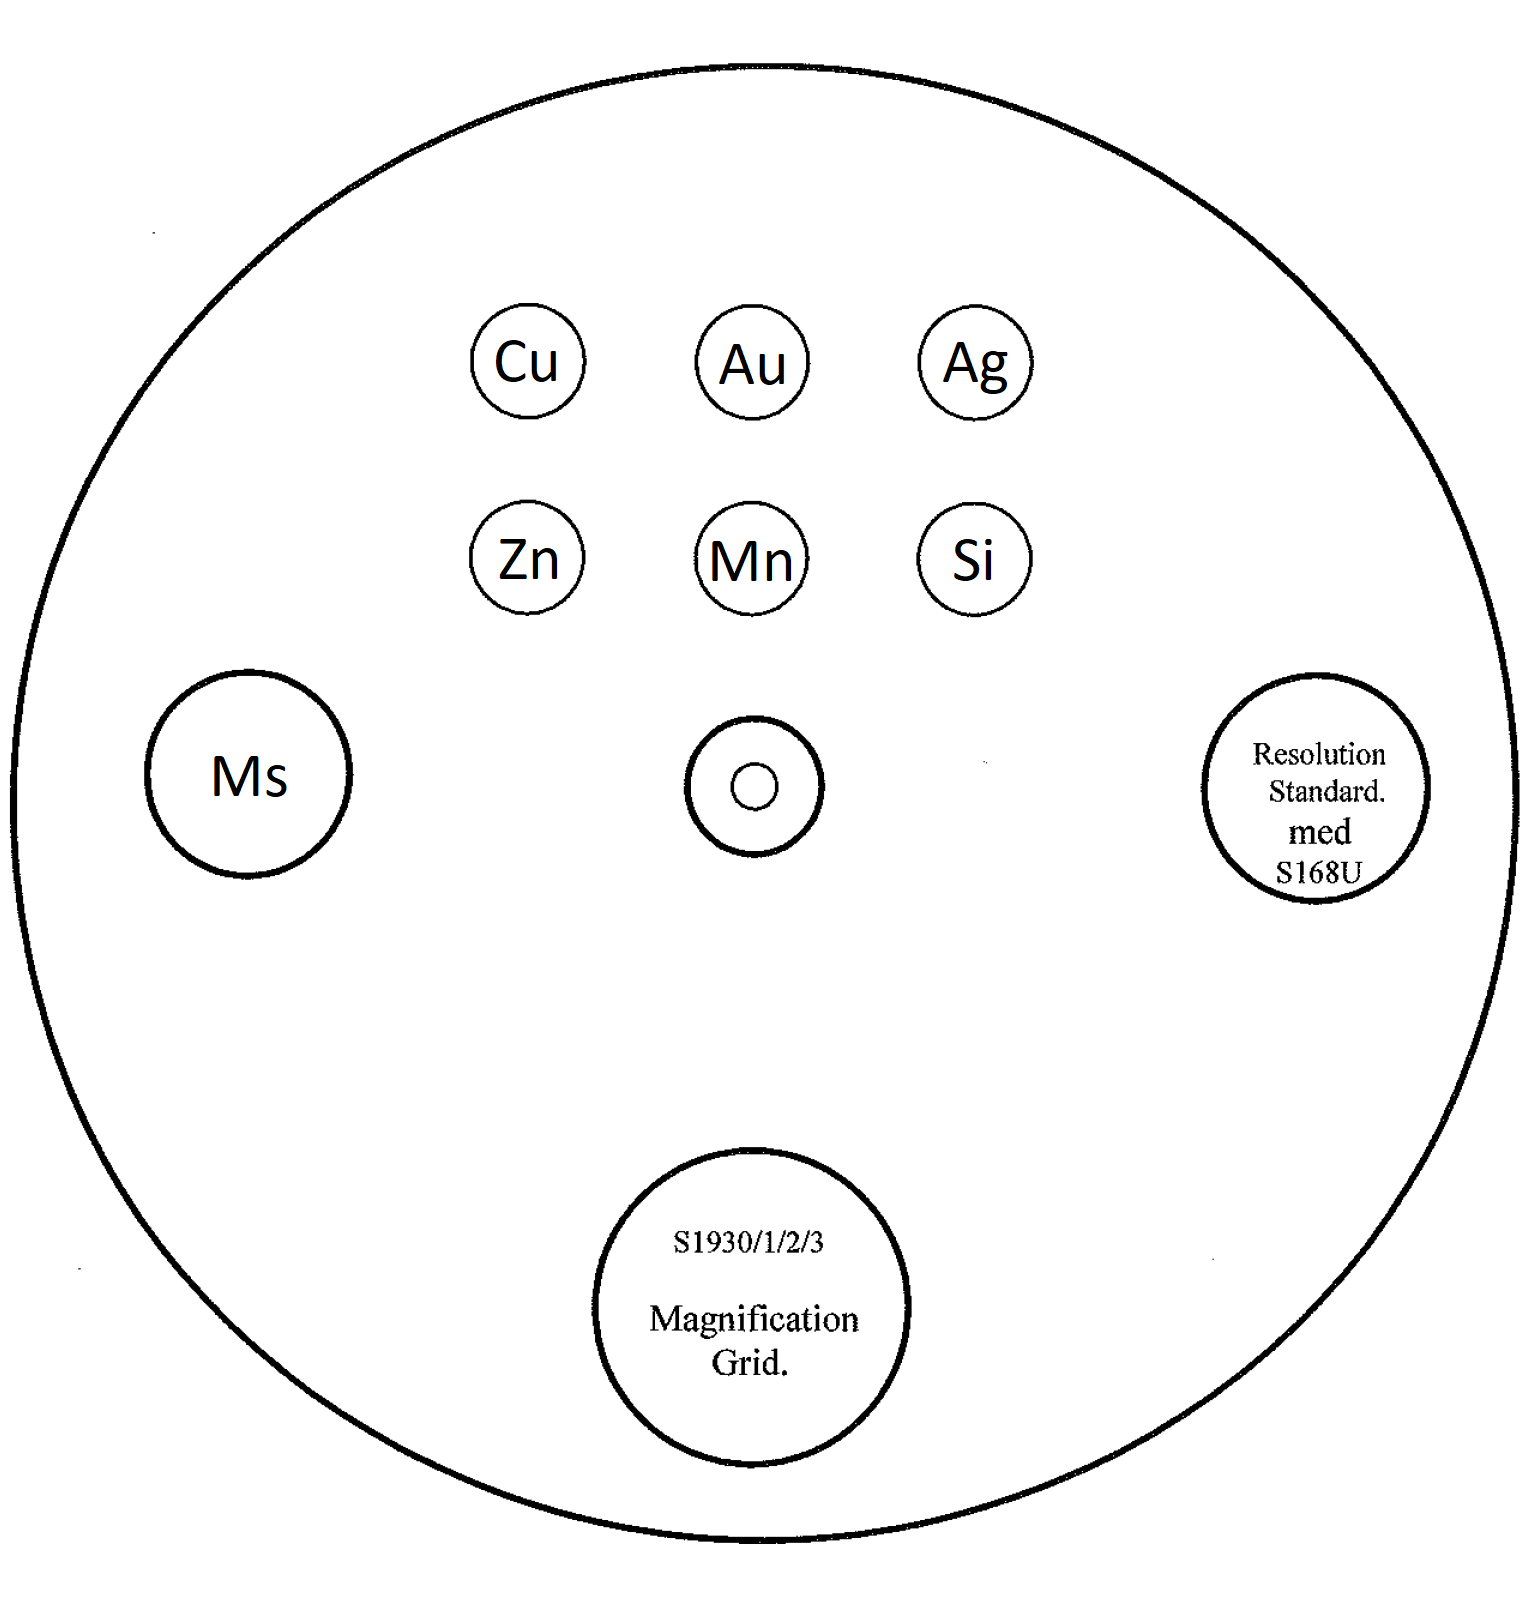
\includegraphics[width=.4\textwidth]{img/Messingprobe}
		\caption{Schematische Darstellung der Halterung mit unterschiedlichen Proben.\cite{wwu}}
		\label{fig:messing_halterung}
	\end{wrapfigure}
	Um nur das Röntgen-Absorptionsspektrum einer bestimmten Probe aufzunehmen, wird nur der Bereich, welcher von Interesse ist, abgebildet.
	Dafür wird die zu untersuchende Probe innerhalb des Mikroskops in den Mittelpunkt des Elektronenstrahls gefahren und die Vergrößerung erhöht, damit nur eine Legierung bzw. ein Element sichtbar ist.

	\

	In \cref{fig:messing_spektrum} sind die aufgenommen Spektren für Messing, Kupfer und Zink zu erkennen.
	Da für die Bestimmung von Kupfer- und Zinkgehalt hier nur die Charakteristischen $K_\alpha$- und $K_\beta$-Linien relevant sind, sind die gesamten Spektren und Darstellungen der $L$-Linien (\cref{fig:l-linien}) dem Anhang zu entnehmen.
	Letztere sind für die Auswerung nicht geeignet, da dort nicht zwischen $L_\alpha$ und $L_\beta$ unterschieden werden kann.

	Die Verteilung der Datenpunkte um die $K$-Linien werden als gaußförmig angenommen und daher mit Gauß-Funktionen angenähert.
	Als Startparameter dienen die von \cite{brukerPTE} gegebenen Energien für die $K$-Linien von Kupfer und Zink.
	Dargestellt ist dies in \cref{fig:k-linien}.
	\begin{figure}[ht]
		\centering
		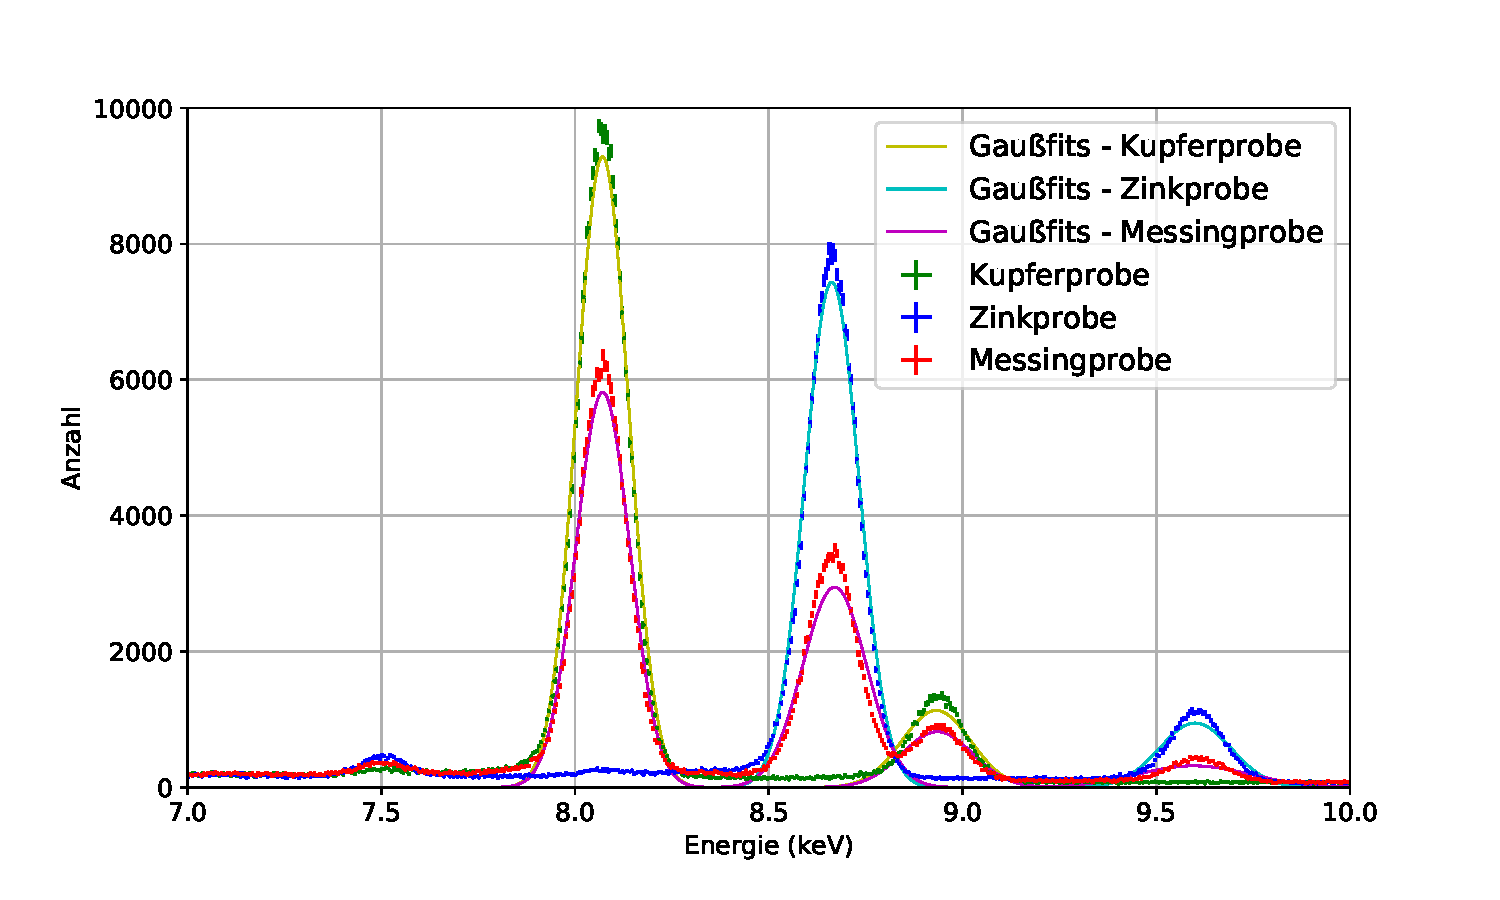
\includegraphics[width=.8\textwidth]{plots/KupferprobeK}
		\caption{Röntgen-Absorptionsspektrum im Bereich der $K$-Linien von Kupfer und Zink für eine Messing-, Kupfer- und Zinkprobe. Zusätzlich dazu Gauß-Annäherungen für die einzelnen Proben und deren charakteristischer Linien.}
		\label{fig:k-linien}
	\end{figure}
	Für die Unsicherheit der Anzahl von $n$ Datenpunkten wird $\sqrt{n}$ verwendet.
	Der direkte Vergleich der Amplituden der Gauß-Annäherungen von Messing zu denen von Kupfer bzw. Zink liefert die in \cref{tab:amplituden} dargestellte Verhältnisse.
	\begin{table}
		\centering
		\caption{Verhältnisse der Amplituden charakteristischer Linien von Messing (Ms) zu Kupfer (Cu) bzw. Zink (Zn).}
		\begin{tabular}{l|c|c|c}
			Verhältnis & $K_\alpha$ & $K_\beta$ & Mittelwert \\ \hline
			% & & & \\
			Ms/Cu & $(62.6\pm3.5)\%$ & $(72.0\pm9.0)\%$ & $(67.0\pm5.0)\%$ \\
			Ms/Zn & $(39.6\pm2.9)\%$ & $(34.0\pm4.0)\%$ & $(36.6\pm2.5)\%$ \\
		\end{tabular}
		\label{tab:amplituden}
	\end{table}

\subsection{Untersuchung unbekannter Elemente} % TODO

\begin{figure}[H]
	\centering
	\begin{subfigure}[c]{.45\textwidth}
		\centering
		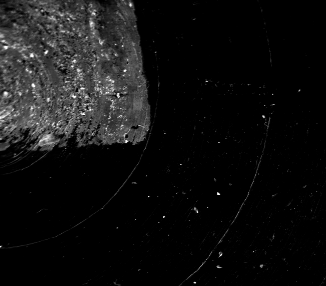
\includegraphics[width=.8\textwidth]{raw/SEM/Map4ProbenExt}
		\subcaption{}
	\end{subfigure}
	\begin{subfigure}[c]{.45\textwidth}
		\centering
		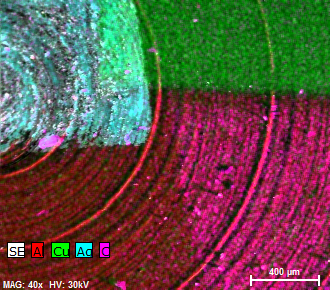
\includegraphics[width=.8\textwidth]{raw/SEM/Mapdaten4Proben}
		\subcaption{}
	\end{subfigure}
	\caption{SEM-Bild der unbekannten Proben.SEM-Bild mit Elementkarte aus den Röntgen-Absorptionsspektren von Silber, Kupfer, Aluminium und Kohlenstoff.EDX Analyse einer unbekannten Probe.} %TODO
	\label{fig:elementalMap}
\end{figure}

	\

	...

\subsection{Diskussion der SEM-Ergebnisse}

	% duplex brass -> \cite{wikiMs} 55-65 Cu / 35-45 Zn
